\chapter{Supply and Demand}

\section{Introduction}

\begin{itemize}

	\item An \underline{economy} is a system of producing, distributing, and consuming goods and services.
	
	\item \underline{Economics} is the study of economies.

	\item \underline{Microeconomics} is the study of how individuals, households, and firms make decisions and how they interact in specific markets.

	\item \underline{Macroeconomics} is the study of society's overall system of production, distribution, and consumption.
	
\end{itemize}

\section{Markets and Competition}

	\begin{itemize}

	\item A \underline{market} is a group of buyers and sellers of a particular good or service.
	
	\item A \underline{competitive market} is a market with so many buyers and sellers that each has a negligible impact on the market price.
	
	\item A market is \underline{perfectly competitive} if:
	
		\begin{enumerate}
	
		\item The goods/services offered for sale are all exactly the same.
		
		\item The buyers and sellers are so numerous that no single buyer/seller has any influence on the market price.
	
		\end{enumerate}
	
	\item Buyers and sellers in perfectly competitive markets are called \underline{price takers} because they must accept the market price. 

	\end{itemize}

\section{Demand}

\subsection{The Demand Curve}

	\begin{itemize}

	\item The \underline{quantity demanded} of a good is the amount that buyers are willing and able to purchase.
	
		\begin{itemize}
		
		\item There are many determinants of quantity demanded, but the most important is the good's price.
		
		\end{itemize}
		
	\item \underline{Law of Demand}: Holding everything else constant, when the price of a good rises, the quantity demanded falls. When the price falls, the quantity demanded rises.
	
	\item A \underline{demand schedule} is a table that shows the relationship between the price of a good and the quantity demanded (holding every other determinant of quantity demanded constant).
	
	\item The \underline{demand curve} is the line relating price and quantity demanded (holding everything else constant).
	
		\begin{itemize}
		
		\item By convention, price is plotted on the $y$-axis and quantity demanded is plotted on the $x$-axis.
		
		\end{itemize}

	\end{itemize}
	
	\underline{Ex.} Catherine's Demand Schedule and Demand Curve
	
	\begin{center}
	\begin{tabular}{ c | c }
	Price of Ice-Cream Cone & Quantity of Cones Demanded \\
	\hline
	\$ 0 & 12 cones \\
	1 & 10 \\
	2 & 8 \\
	3 & 6 \\
	4 & 4 \\
	5 & 2 \\
	6 & 0
	\end{tabular}
	
	\vspace{5mm}
	
	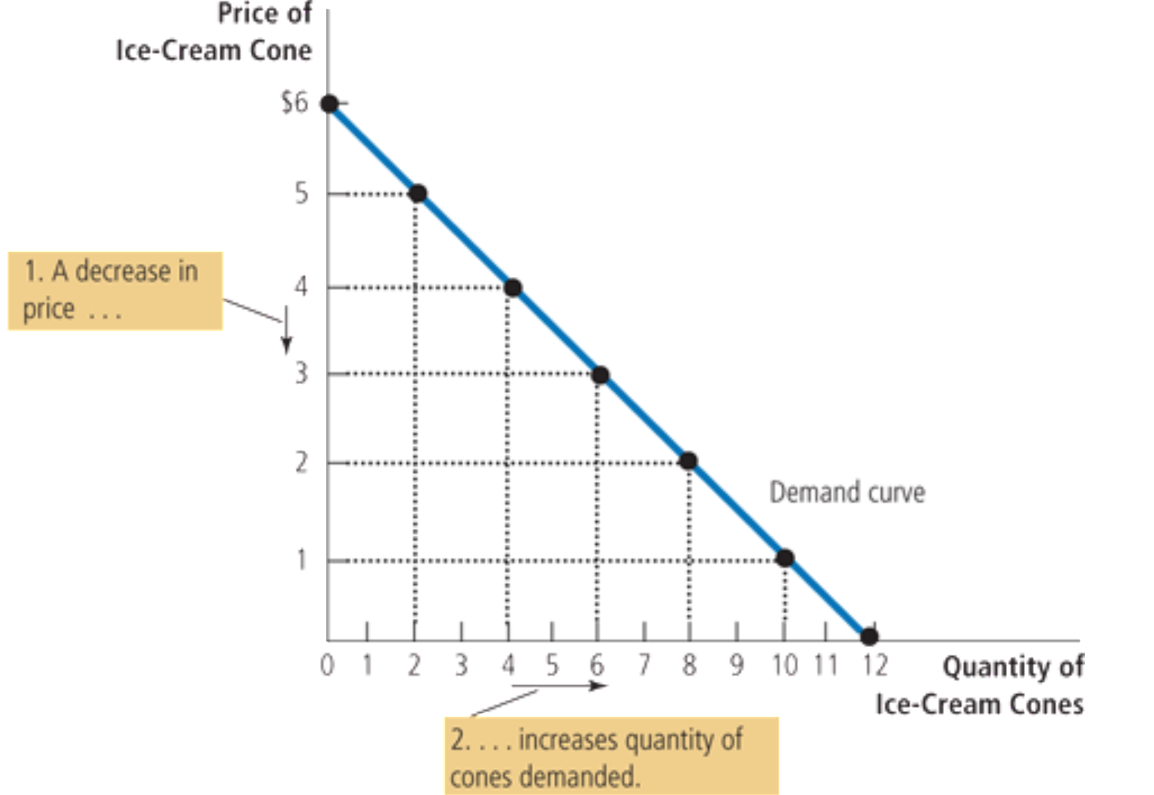
\includegraphics[scale = 0.225]{1.3.1_indiv_d_curve}
	\end{center}
	
\subsection{Market Demand}

	\begin{itemize}
	
	\item The quantity demanded in a market is the sum of every individuals' quantity demanded at each price
	
	\end{itemize}
	
	\underline{Ex.} Market Demand Schedule and Demand Curve
	
	\begin{center}
	
	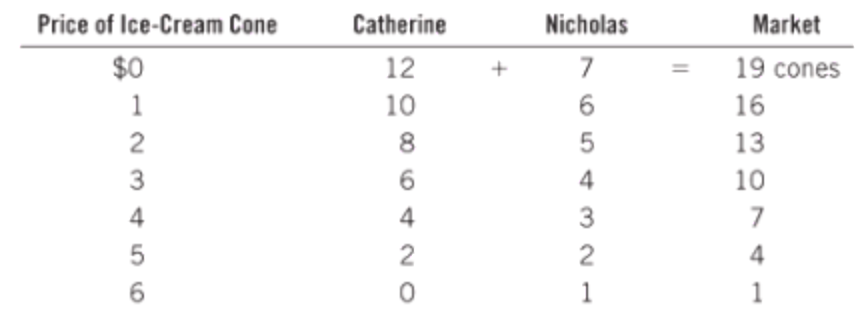
\includegraphics[scale = 0.75]{1.3.2_mkt_d_schedule}
	
	\vspace{5mm}
	
	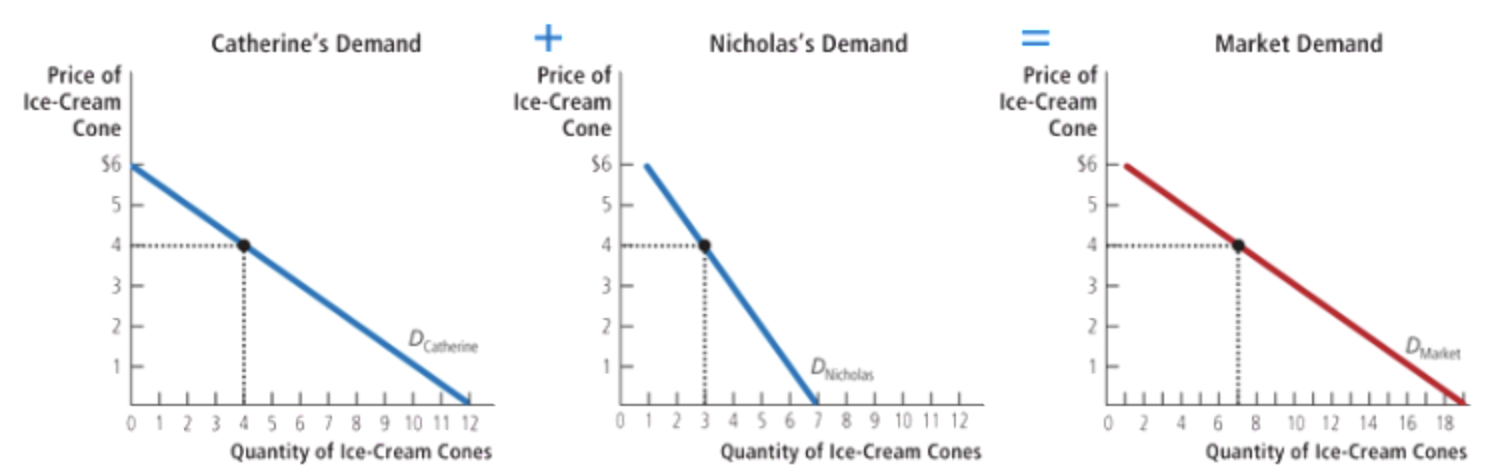
\includegraphics[scale = 0.5]{1.3.2_mkt_d_curve}
	
	\end{center}
	
\subsection Shifts in the Demand Curve

	\begin{itemize}

	\item

	\end{itemize}


